\chapter{Extração de Dados}
\label{cap:Extracao}

Para a extração dos dados para a análise de sentimentos foi criado um
\textit{crawler} ou robô de navegação. Esse robô tem como objetivo a navegação
automática no conteúdo web do Reddit, extraindo os dados referentes a tópicos e
a comentários e persistindo esses em um banco de dados.

\section{\textit{Crawler}}

O \textit{Crawler} foi escrito na linguagem Java por se tratar de uma linguagem
com uma grande quantidade de bibliotecas disponíveis e também
sua facilidade de implementação. A Figura \ref{fig:crawler} representa a
arquitetura utilizada para desenvolvimento deste software.

\begin{figure}[htbp]
\centering
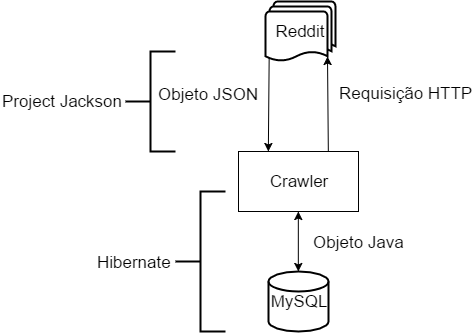
\includegraphics[height=225px]{imagens/arquitetura.png}
\caption{Arquitetura do \textit{Crawler}}
\label{fig:crawler}
\end{figure}

A partir de um \textit{link} para um tópico, o software tem como tarefa, a
extração e pesquisa de dados relacionados com o tópico em questão. Isso se faz
da seguinte forma, primeiramente, é enviada uma requisição para o \textit{link}
utilizando o sufixo ``.json'', de forma demonstrada na API, a partir dessa
requisição, o \textit{website} retorna um objeto \ac{JSON}.

Como o \ac{JSON} possui 68 campos que assim como seus tipos de dados, não se
encontram em nenhuma documentação, foi utilizado o \textit{website}
jsonschema2pojo\footnote{http://www.jsonschema2pojo.org/} para mapear o \ac{JSON} retornado em um
objeto Java. Esse \textit{website} tem como objetivo a conversão de um esquema \ac{JSON} ou o próprio \ac{JSON} para um \ac{POJO} ou Os Singelos Clássicos Objetos Java, permitindo
o \textit{download} da classe para utilização, já com as anotações
``@JsonProperty'' utilizadas na biblioteca Jackson. Este objeto disponibilizado a
partir do \textit{website} foi renomeado para \textit{RedditPost} e adicionado
ao código fonte da aplicação.

A anotação ``@JsonProperty'' é relativa ao
mapeamento do objeto Java com relação ao \ac{JSON} e nos permite com
intermédio da classe \textit{Object Mapper} instanciar o objeto
\textit{RedditPost} a partir de um objeto \textit{String} em formato \ac{JSON}.

\begin{lstlisting}
RedditPost post = objectMapper.readValue(iteratorPost.get("data").toString(),
RedditPost.class);
\end{lstlisting}

Utilizando o método \textit{readValue} que tem como retorno um \textit{Object},
é informado um objeto \textit{String}, neste caso
\textit{``iteratorPost.get("data").toString()"} e uma classe mapeada, neste caso
\textit{RedditPost}.

Porém, para o correto funcionamento, deve ser feita a seguinte mudança: O campo
\textit{edited} representando se foi editado o comentário, retornado no
\ac{JSON} apresenta um tipo de dado ambíguo aonde que caso o comentário não tenha sido editado, ele apresenta o valor \textit{booleano} de \textit{false}, porém, ao ter sido editado, ele apresenta
seu valor em um formato decimal. Este e demais objetos que apresentavam o tipo
de dado de forma ambígua foram transformados em objetos \textit{String}.


A partir deste objeto Java, foi utilizado o \textit{framework} Hibernate para a
criação do banco de dados, assim como persistência destes. Através da anotação
``@Entity'', adicionada também na classe RedditPost. O Hibernate mapeia essa
entidade junto ao banco de dados, neste caso, MySQL.

Para criação das tabelas do banco de dados, foi utilizada a propriedade
\textit{hibernate.hbm2ddl.auto} do Hibernate. Essa propriedade quando
instânciada uma nova sessão do \textit{framework} no Java executa as seguintes
ações dependendo de seus valores informados:


\begin{itemize}
  \item \textit{validate}: Não efetua mudanças no banco de dados, somente
  valida.
  \item \textit{update}: Atualiza o esquema do banco de dados conforme os
  objetos mapeados na camada Java.
  \item \textit{create}: Cria o esquema contendo tabelas e campos a partir dos
  objetos Java, destruindo dados anteriores.
  \item \textit{create-drop}: Cria o esquema da mesma que o \textit{create},
  porém, ao termino da sessão, remove o esquema criado.
\end{itemize}

No primeiro momento, a propriedade obteve o valor \textit{create}, para fins de
criação e validação do esquema criado e após isso, foi informado \textit{update}
como seu valor para tornar reflexo as alterações feitas na camada Java.

Portanto, a execução do \textit{Crawler} funciona da seguinte forma, é enviada
uma requisição para o \textit{website} através da URL do tópico em questão com o
sufixo ``\textit{.json}'' no final. O \textit{website} retorna um
\textit{JSON} com os dados referentes ao tópico solicitado e aos comentários
deste tópico. Este objeto \ac{JSON} é convertido em um \ac{POJO} através da
biblioteca Jackson e persistida no banco de dados através do \textit{framework}
Hibernate. Como a API do Reddit possui uma restrição do número de comentários
disponibilizados, são efetuadas novas requisições para a seção \textit{``more''}
disponível no \ac{JSON} de retorno.

\section{Tópicos Selecionados}

Para análise de sentimentos e comparação dos resultados obtidos, foram
selecionados 25 tópicos controversos, selecionados com o objetivo de encontrar
padrões de opinião entre seus comentários, distribuídos da seguinte forma:

Tópicos relacionados com o cenário político nacional:
\begin{itemize}
  \item
  \textit{Brazil Seeks To Copy U.S. Gun Culture ``to allow embattled
  citizens the right to defend themselves from
  criminals''} - Disponível em: 
  \url{https://www.reddit.com/r/worldnews/comments/36ny58/brazil_blogger_known_for_reporting_on_corruption/}.
  \item
  \textit{Brazil descends into chaos as Olympics looms} - Disponível em: 
  \url{https://www.reddit.com/r/worldnews/comments/4bqcc3/brazil_descends_into_chaos_as_olympics_looms/}.
  \item
  \textit{Plane carrying Brazil Supreme Court judge crashes into sea}
   - Disponível em: \url{https://www.reddit.com/r/worldnews/comments/5oyz3b/plane_carrying_brazil_supreme_court_judge_crashes/}.
  \item
  \textit{Brazil passes Internet governance Bill: Brazil has made history with
  the approval of a post-Snowden Bill which sets out principles, rights and guarantees for Internet users.} - Disponível em: \url{https://www.reddit.com/r/worldnews/comments/21f3as/brazil_passes_internet_governance_bill_brazil_has/}.
  \item
  \textit{FIFA generated more than \$4 billion in sales from the 2014 World Cup,
  and is Giving Brazil \$100 Million After The Country Spent \$15 Billion On The
  World Cup} - Disponível em: \url{https://www.reddit.com/r/worldnews/comments/2t65ql/fifa_generated_more_than_4_billion_in_sales_from/}.
  \item
  \textit{Brazil Seeks To Copy U.S. Gun Culture "to allow embattled citizens the
  right to defend themselves from
  criminals"} - Disponível em: \url{https://www.reddit.com/r/worldnews/comments/3skpe7/brazil_seeks_to_copy_us_gun_culture_to_allow/}.
\end{itemize}

Tópicos relacionados sobre política internacional.
\begin{itemize}
  \item
  \textit{2.6 terabyte leak of Panamanian shell company data reveals "how a
  global industry led by major banks, legal firms, and asset management companies
  secretly manages the estates of politicians, Fifa officials, fraudsters and
  drug smugglers, celebrities and professional
  athletes."}. - Disponível em: \url{https://www.reddit.com/r/worldnews/comments/4d75i7/26_terabyte_leak_of_panamanian_shell_company_data/}.
  \item
  \textit{Fidel Castro is dead at
  90.} - Disponível em: \url{https://www.reddit.com/r/worldnews/comments/5exz2e/fidel_castro_is_dead_at_90/}.
  
  \item
  \textit{Donald Trump to strip all funding from State Dept team promoting women's rights around the world - Leaked plan comes as First Daughter Ivanka defends her father's record with women} - Disponível em: \url{https://www.reddit.com/r/worldnews/comments/67ivae/donald_trump_to_strip_all_funding_from_state_dept/}.
  
  \item
  \textit{Manchester Arena 'explosions': Two loud bangs heard at MEN Arena} - Disponível em: \url{https://www.reddit.com/r/worldnews/comments/6cqdye/manchester_arena_explosions_two_loud_bangs_heard/}.
  
  \item
  \textit{Sweden asks the U.S. to explain Trump comment on
  Sweden} - Disponível em: \url{https://www.reddit.com/r/worldnews/comments/5uzetf/sweden_asks_the_us_to_explain_trump_comment_on/}
  
  \item\textit{“Canada will welcome you,” Trudeau invites refugees as Trump bans
  them} - Disponível em: \url{https://www.reddit.com/r/worldnews/comments/5qqa51/canada_will_welcome_you_trudeau_invites_refugees/}
\end{itemize}

Tópicos diversos.
\begin{itemize}
  \item
  \textit{I’m Bill Gates, co-chair of the Bill \& Melinda Gates Foundation. Ask
  Me Anything.} - Disponível em: \url{https://www.reddit.com/r/IAmA/comments/5whpqs/im_bill_gates_cochair_of_the_bill_melinda_gates/}.
  \item
  \textit{Hey, it's Lars from Metallica. AMA} - Disponível em: \url{https://www.reddit.com/r/IAmA/comments/1wl9ic/hey_its_lars_from_metallica_ama/}.
  
  \item
  \textit{I'm the CEO of Renault and Nissan and we're making autonomous driving vehicles happen by 2020. Ask me anything!} - Disponível em: \url{https://www.reddit.com/r/IAmA/comments/2s7obx/im_the_ceo_of_renault_and_nissan_and_were_making/}.
  
  \item
  \textit{I am Julian Assange founder of WikiLeaks -- Ask Me Anything} - Disponível em: \url{https://www.reddit.com/r/IAmA/comments/5n58sm/i_am_julian_assange_founder_of_wikileaks_ask_me/}.
  
\end{itemize}


A partir destes tópicos selecionados, foram extraídos seus dados, como conteúdo,
usuário de criação e número de \textit{upvotes}. Somente foram extraídos
comentários em resposta ao tópico em questão, comentários em resposta a outros
comentários foram desconsiderados pois estes podem não estar relacionados com o
tópico em questão, o que torna a sua análise de sentimento inaproveitável. Além
de não existirem \textit{softwares} ou \textit{frameworks} preparados para a
análise de sentimentos de uma conversa sobre um determinado tópico.
